% \documentclass[../main.tex]{subfiles}
% \begin{document}

\thispagestyle{myheadings}

\chapter{Neural Signals: Computational considerations, interpretation and usage}
\label{sec:neural-signals}

\section{Image Processing}\label{sec:image-processing}

The entire procedure for processing images and extracting cell signals can be performed in substantially less time than most commonly available tools using the approach described in Aim 1, particularly the methods for restricting the spatial extent of pixel-association operations, and distributing operations across parallel processing cores using a Single Program Multiple Data (SPMD) archetype.
However, the total time still exceeds that of the acquisition session.
Inefficiency arises from the overhead involved with distributing data and passing information between separate parallel processes.
Graphics cards, however execute in what's called Single Instruction Multiple Data (SIMD) fashion, to distribute computation across the thousands of processing cores.

The processing components are implemented using the MATLAB System-Object framework, which allows for slightly faster performance through internal optimizations having to do with memory allocation.
Most system objects, each representing one step in the serial processing and signal-extraction procedure, also have companion functions that implement the computation-heavy components of each algorithm using a pre-compiled CUDA kernel.

\subsection{Benchmarking \& General Performance}\label{sec:benchmarking-general-performance}

Built-in MATLAB functions that execute on the GPU can be profiled with benchmarking functions like \emph{gputimeit()}, or with the \emph{tic/toc} functions.
When execution isn't fast enough, they need to be replaced with custom functions.
The custom functions typically achieve the speed up necessary by enabling the operation to carried out on several frames at once.
This reduces the over-head costs inposed for each function call by spreading it over several frames.
This solution is not ideal, as it increases the latency of solutions, however does not preclude implementation in real-time system if the procedures are adapted to run on a real-time hybrid system-on-module like NVIDIA's Tegra X1, which should involve minimal effort once a standard set of successful procedures is realized.
The current implementation tests the processing time of each stage of the process to ensure that the sum is less than the acquisition time for each frame dictated by the inverse of the frame-rate (30-50 milliseconds).

\subsection{Buffered Operations}\label{sec:buffered-operations}

Combining frames for each operation can result in near linear speedup.
For example, for the phase-correlation step required for motion correction, the FFT and IFFT are called on 16 image-frames at once, and the time take to accomplish is approximately the same as if the operation were called on 1 frame.
This essentially leads to a 16x speedup, though the latency is also increased slightly.
The best size to use is difficult to pre-determine, and typically must be measured for varying size `chunks' using the benchmarking functions indicated above.
The system objects manage the details necessary to allow buffered chunks of video to be passed to each stage without introducing artifacts at the temporal edges between chunks.

\begin{figure}[htb]\centering
	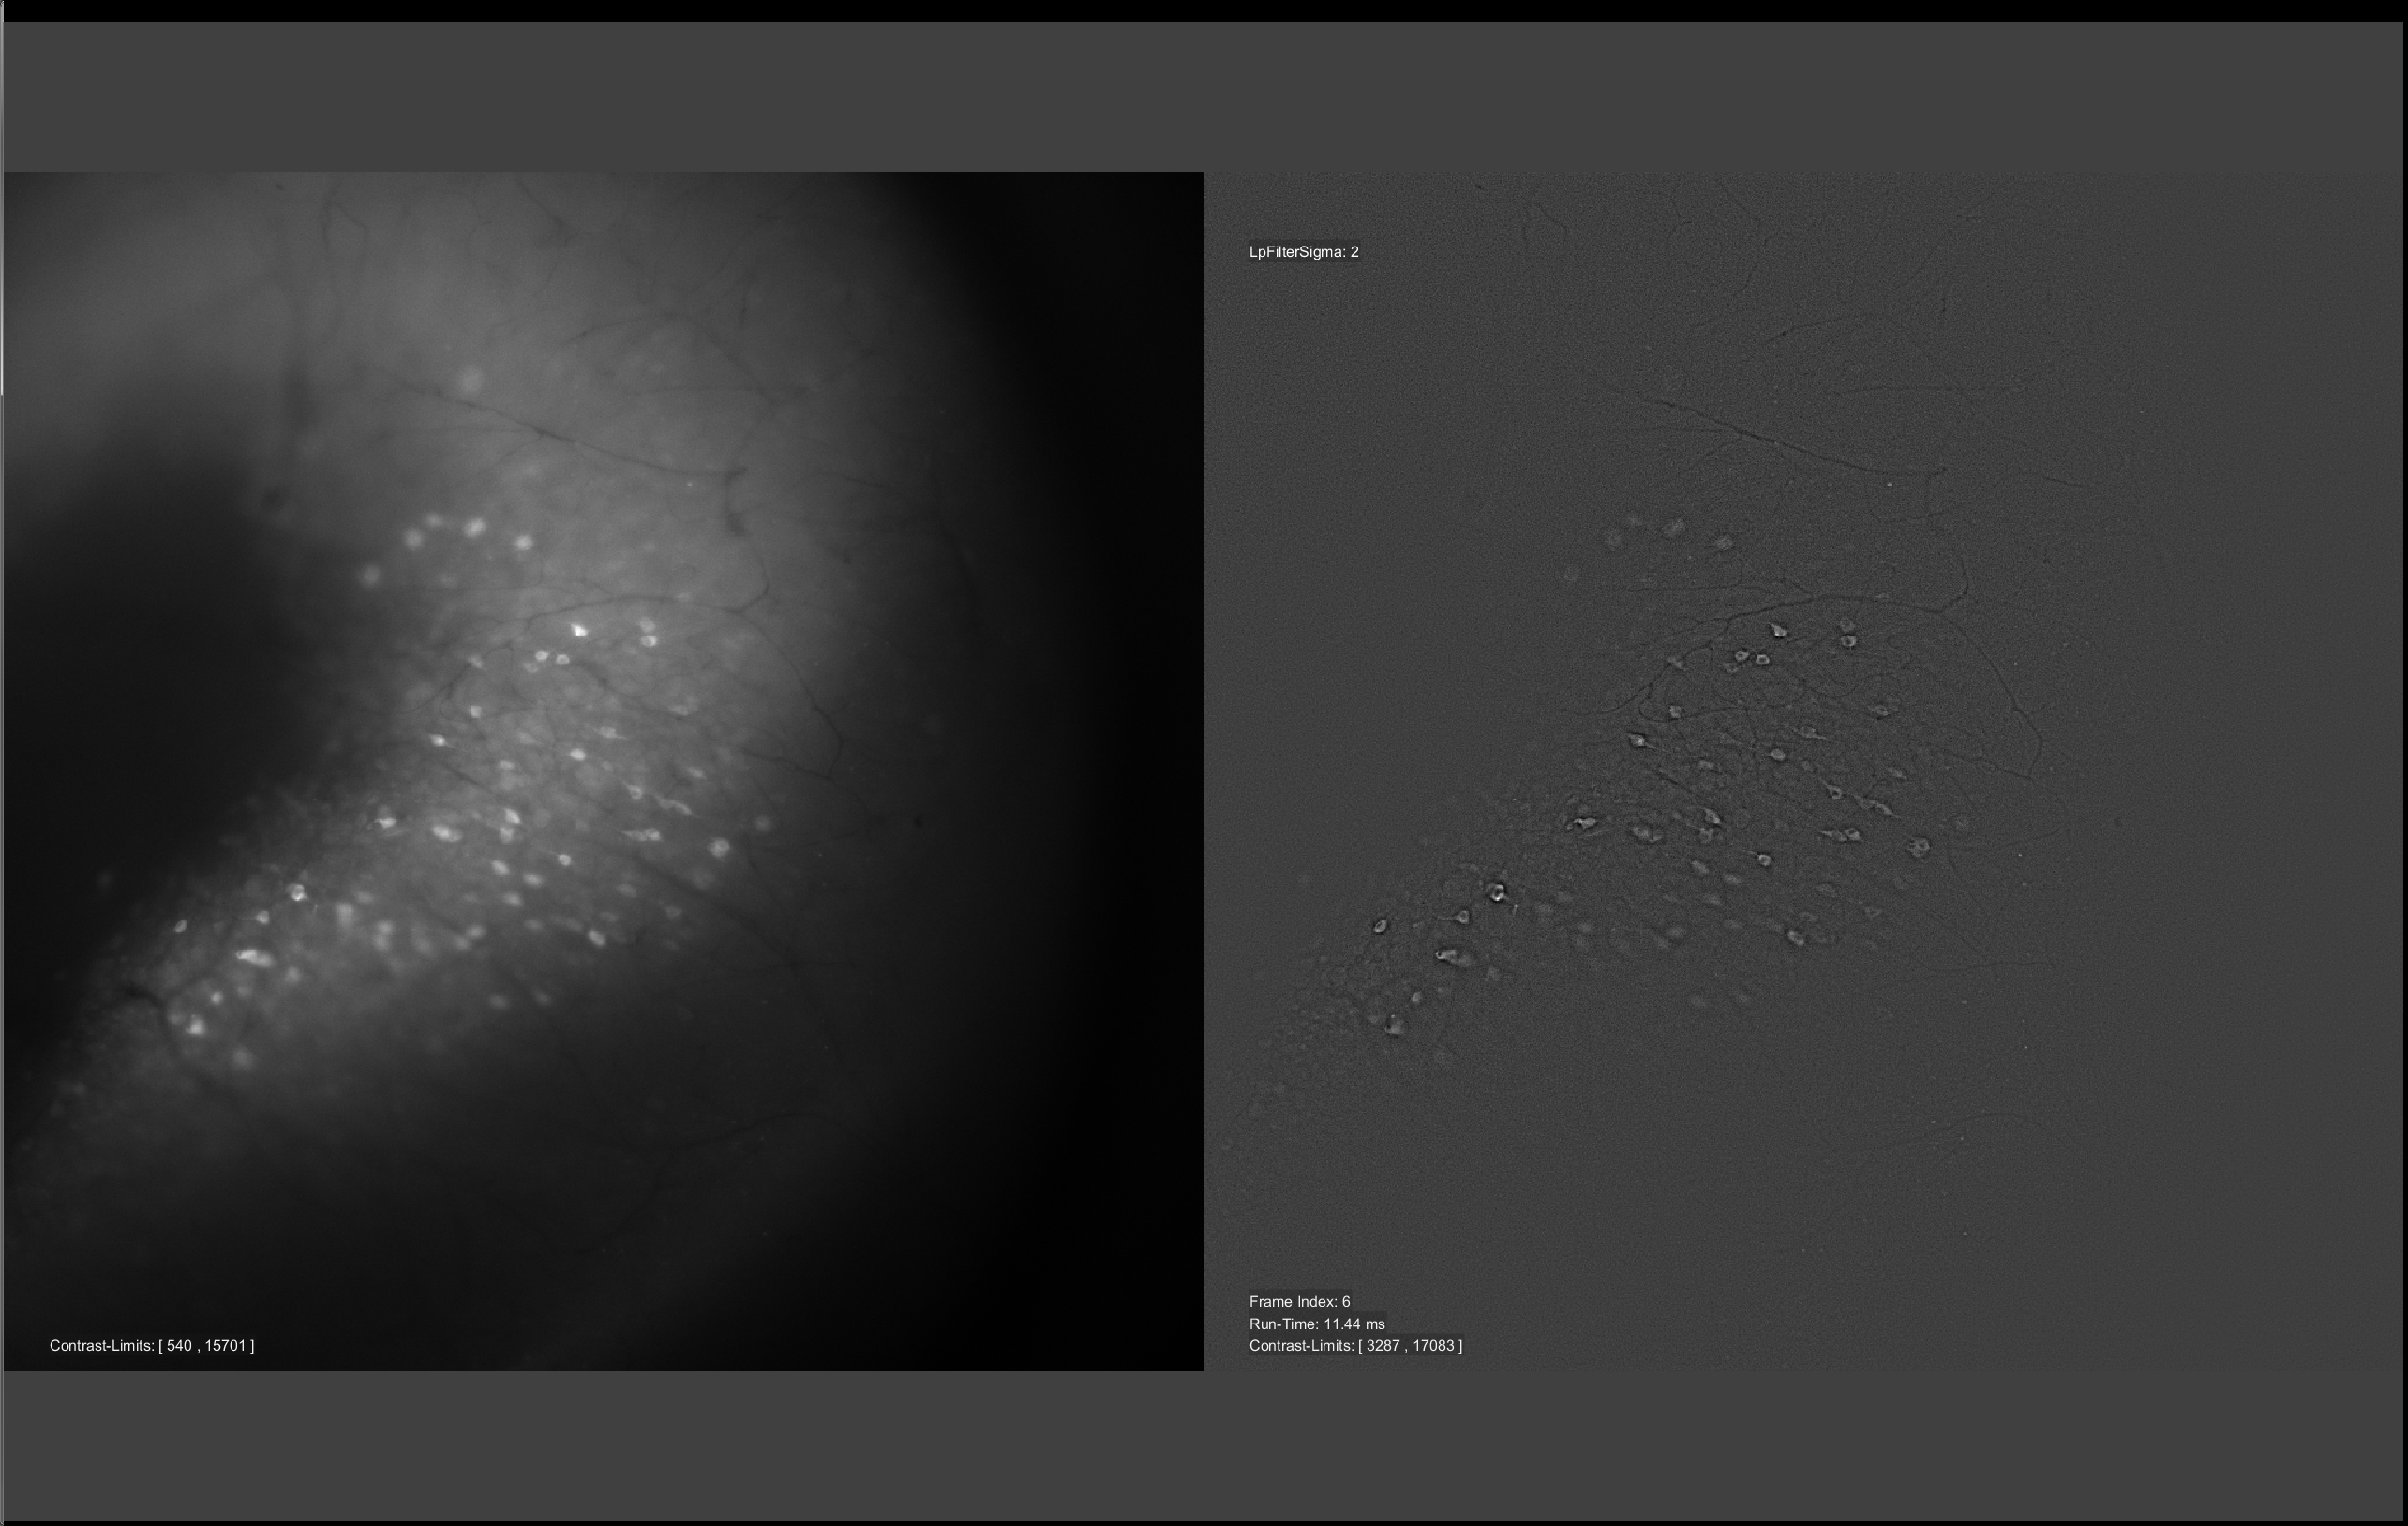
\includegraphics[width=12cm]{figures/screenshot_20150608180058.png}
	\caption{Interactive parameter adjustment for homomorphic filter operation (local contrast enhancement)}
\end{figure}

\subsection{Image Pre-Processing \& Motion Correction}\label{sec:image-pre-processing-motion-correction}

Pre-processing is implemented as with the offline procedure, with a few changes.
Images are aligned in chunks, and they are aligned sequentially to two templates.
One template is the most recent stable frame from the preceding chunk.
The other is a recursively temporal-low-pass filtered image that mitigates slow drifts.
Aligning to the first template is usually more stable as the brightness of cells in the recent image will be more similar to those in the current chunk than will be the brightness of cells in the slow-moving average.

The displacement of each frame is found to sub-pixel precision, then used with a custom bicubic resampling kernel that replaces any pixels at the edges with images from the moving average.



\begin{figure}[htb]\centering
	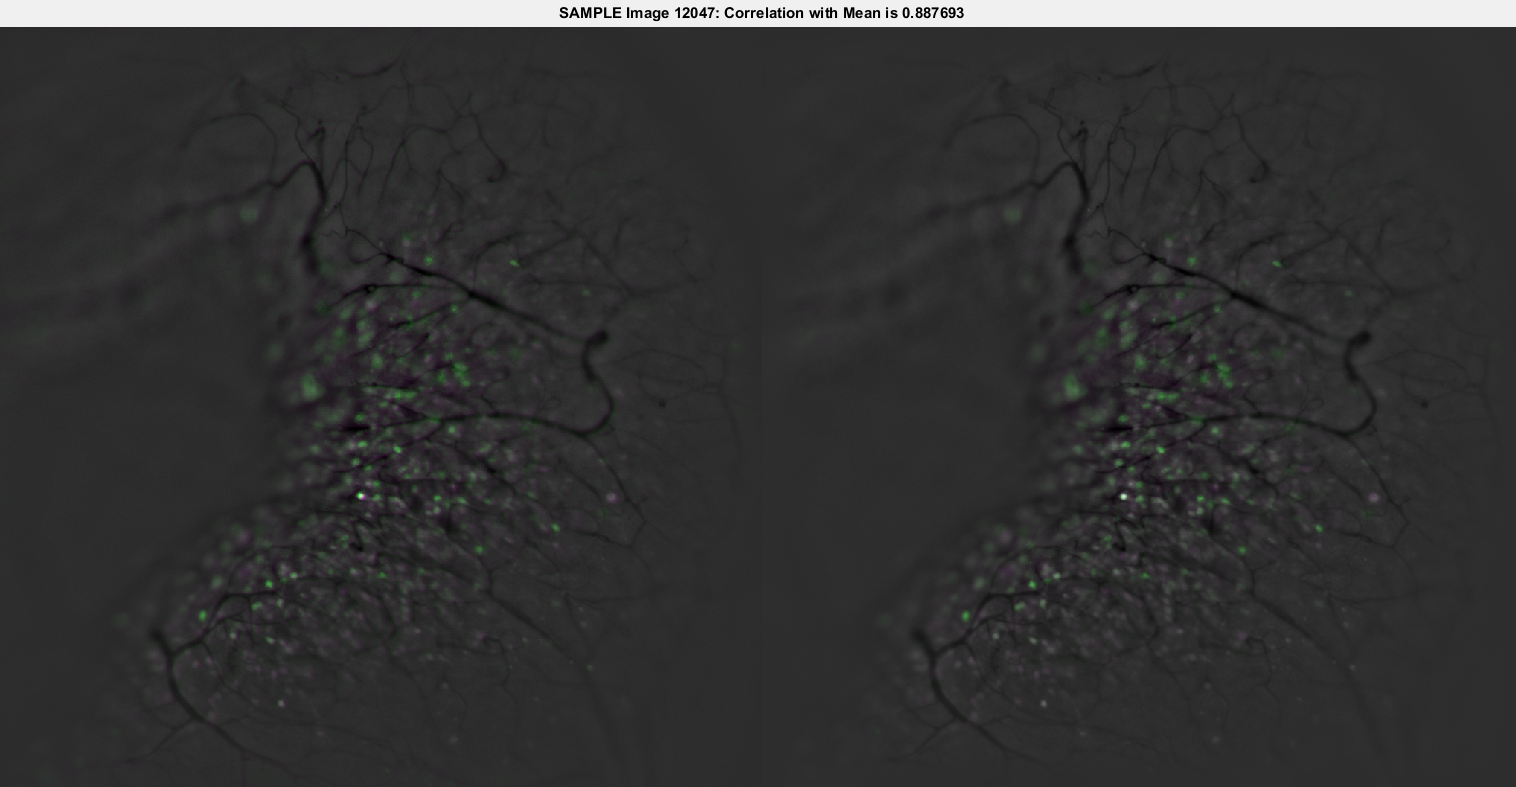
\includegraphics[width=12cm]{figures/motion_correction_sample.png}
	\caption{Motion compensated; comparison of uncompensated and compensated frames overlayed with mean image}
\end{figure}

\subsection{Sequential Statistics}\label{sec:sequential-statistics}

A number of statistics for each pixel are updated online and can be used for normalization and segmentation procedures later in the process.
These include the minimum and maximum pixel intensity, and the first four central moments, which are easily converted to the mean, variance, skewness, and kurtosis.
The formulas for making these calculations are given below, and are performed in a highly efficient manner as data are kept local to each processing core, and repeat computations are minimized.
Code implementing these incrental pixel-wise statistic updates in MATLAB is shown in below \ref{lst:update-statistic-gpu}.

Furthermore, the value used to update each central moment at each point in time can be used as a measure of change in the distribution of each pixel caused by the current pixel intensity, as explained next.

\subsubsection{Non-Stationarity \& Differential Moments}\label{sec:non-stationarity-differential-moments}

Stationary refers to the property of a signal such that its statistics do not vary over time, i.e.~its distribution is stable.
Neural signals tend to specifically \emph{not} have this property, in contrast to other measurable components such as those contributed by physiologic noise (heart-rate, respirations, etc.)
.
Thus, by analyzing the evolution of statistical measures calculated for each pixel as frames are added in sequence gives a highly sensitive indicator of neural activity.
This is done using a routine analogous to that for updating central moments given above, except the values returned are not only the updated moment, but also the updating component -- essentially the partial derivative with respect to time.
This is illustrated below, including the normalization functions which convert the partial-moment values to their variance, skewness, and kurtosis analogues:


These functions run on images representing the image intensity, and also on images taken from sequential differences indicating the temporal derivative of image intensity.
The combination of outputs from these operations indicate both when image intensities are significantly high relative to past distribution, and also when intensities are changing significantly faster than learned from their past distribution.


\begin{listing}[ht]
\begin{minted}{matlab}
function [fmin,fmax,m1,m2,m3,m4,n] = statUpdateKernel(f,fmin,fmax,m1,m2,m3,m4,n)

    % update sample count for this pixel
    n = n + 1;

    % precompute & cache some values for speed
    d = f - m1;
    dk = d/n;
    dk2 = dk^2;
    s = d*dk*(n-1);

    % update central moments
    m1 = m1 + dk;
    m4 = m4 + s*dk2*(n.^2-3*n+3) + 6*dk2*m2 - 4*dk*m3;
    m3 = m3 + s*dk*(n-2) - 3*dk*m2;
    m2 = m2 + s;

    % update min & max
    fmin = min(fmin, f);
    fmax = max(fmax, f);

end
\end{minted}
\caption[Incremental update of the pixel statistics (min, max, and first 4 central moments)]{Incremental update of the pixel statistics (min, max, and first 4 central moments). This function can be called to efficiently run in parallel across CPU or GPU cores}
\label{lst:update-statistic-gpu}
\end{listing}

This type of function is also easily translated to stencil functions on for computation on the GPU.


\subsection{Surface Classification: Peaks, Edges, Curvature}\label{sec:surface-classification-peaks-edges-curvature}

Edge-finding methods are employed for establishing boundaries between cells, and first and second-order gradients are used to compute local measures of curvature from an eigenvalue decomposition of the local Hessian matrix.
I won't go into detail, as the utility of these procedure in the most recent implementation has been lost, but nevertheless, the operation is optimized and ready to be plugged back in when further development calls for better accuracy informing cell-segmentation, or when a faster or more accurate motion-correction algorithm is called for.

\subsection{Online Cell Segmentation \& Tracking}\label{sec:online-cell-segmentation-tracking}

Cells are segmented by first running sequential statistics on the properties of identifiable regions on a pixel-wise basis.
That is, as regions are identified in a method similar to that used offline in Aim 1, the region-properties are calculated (Centroid, Bounding-Box, etc.) and statistics for these properties are updated at each pixel covered by a proposed region.
After sufficient evidence has gathered, Seeds are generated by finding the local peak of a seed-probability function that optimizes each pixel's proximity to a region centroid, and distance from any boundary.
Regions are grown from these seed regions, and registered in a hierarchy that allows for co-labeling of cellular and sub-cellular components.
Newly identified regions occur as new seeds, where as seeds overlapping with old regions are used to identify sub-regions, or to track regions over time.

\subsection{Signal Extraction from Subcellular Compartments}\label{sec:signal-extraction-from-subcellular-compartments}

I also have functions for the extraction of normalized Pointwise-Mutual-Information (nPMI), which can operate on a pixel-to-pixel basis or on a region-to-pixel basis.
This operation accumulates mutually informative changes in all pixels in the maximal bounding-box (e.g.~64x64 pixels) surrounding each identified regions centroid.
The weights given by this function can take on values between -1 and 1, and can be used to inform any reduction operations to follow.
Additionally, spatial moments can indicate the subcellular distribution of activity across the identified region.
In this context, the first spatial moment M\textsubscript{00} indicates the mean signal intensity.


\subsection{User Interface for Parameter Tuning}\label{sec:user-interface-for-parameter-tuning}

Some system-objects also incorporate a user interface to aid in parameter selection for tuning.

\subsection{Image Processing: Tone mapping and Filtering}\label{sec:image-processing-tonemapping-and-filtering}
\begin{figure}[htb]\centering
	\includegraphics[height=12cm]{figures/sw-video-processing-feature-generation.png}
	\caption{Feature generation showing complex-valued moving average of distance of each pixel to bounding box corners (post segmentation)}
\end{figure}

% \begin{figure}[htb]\centering
% 	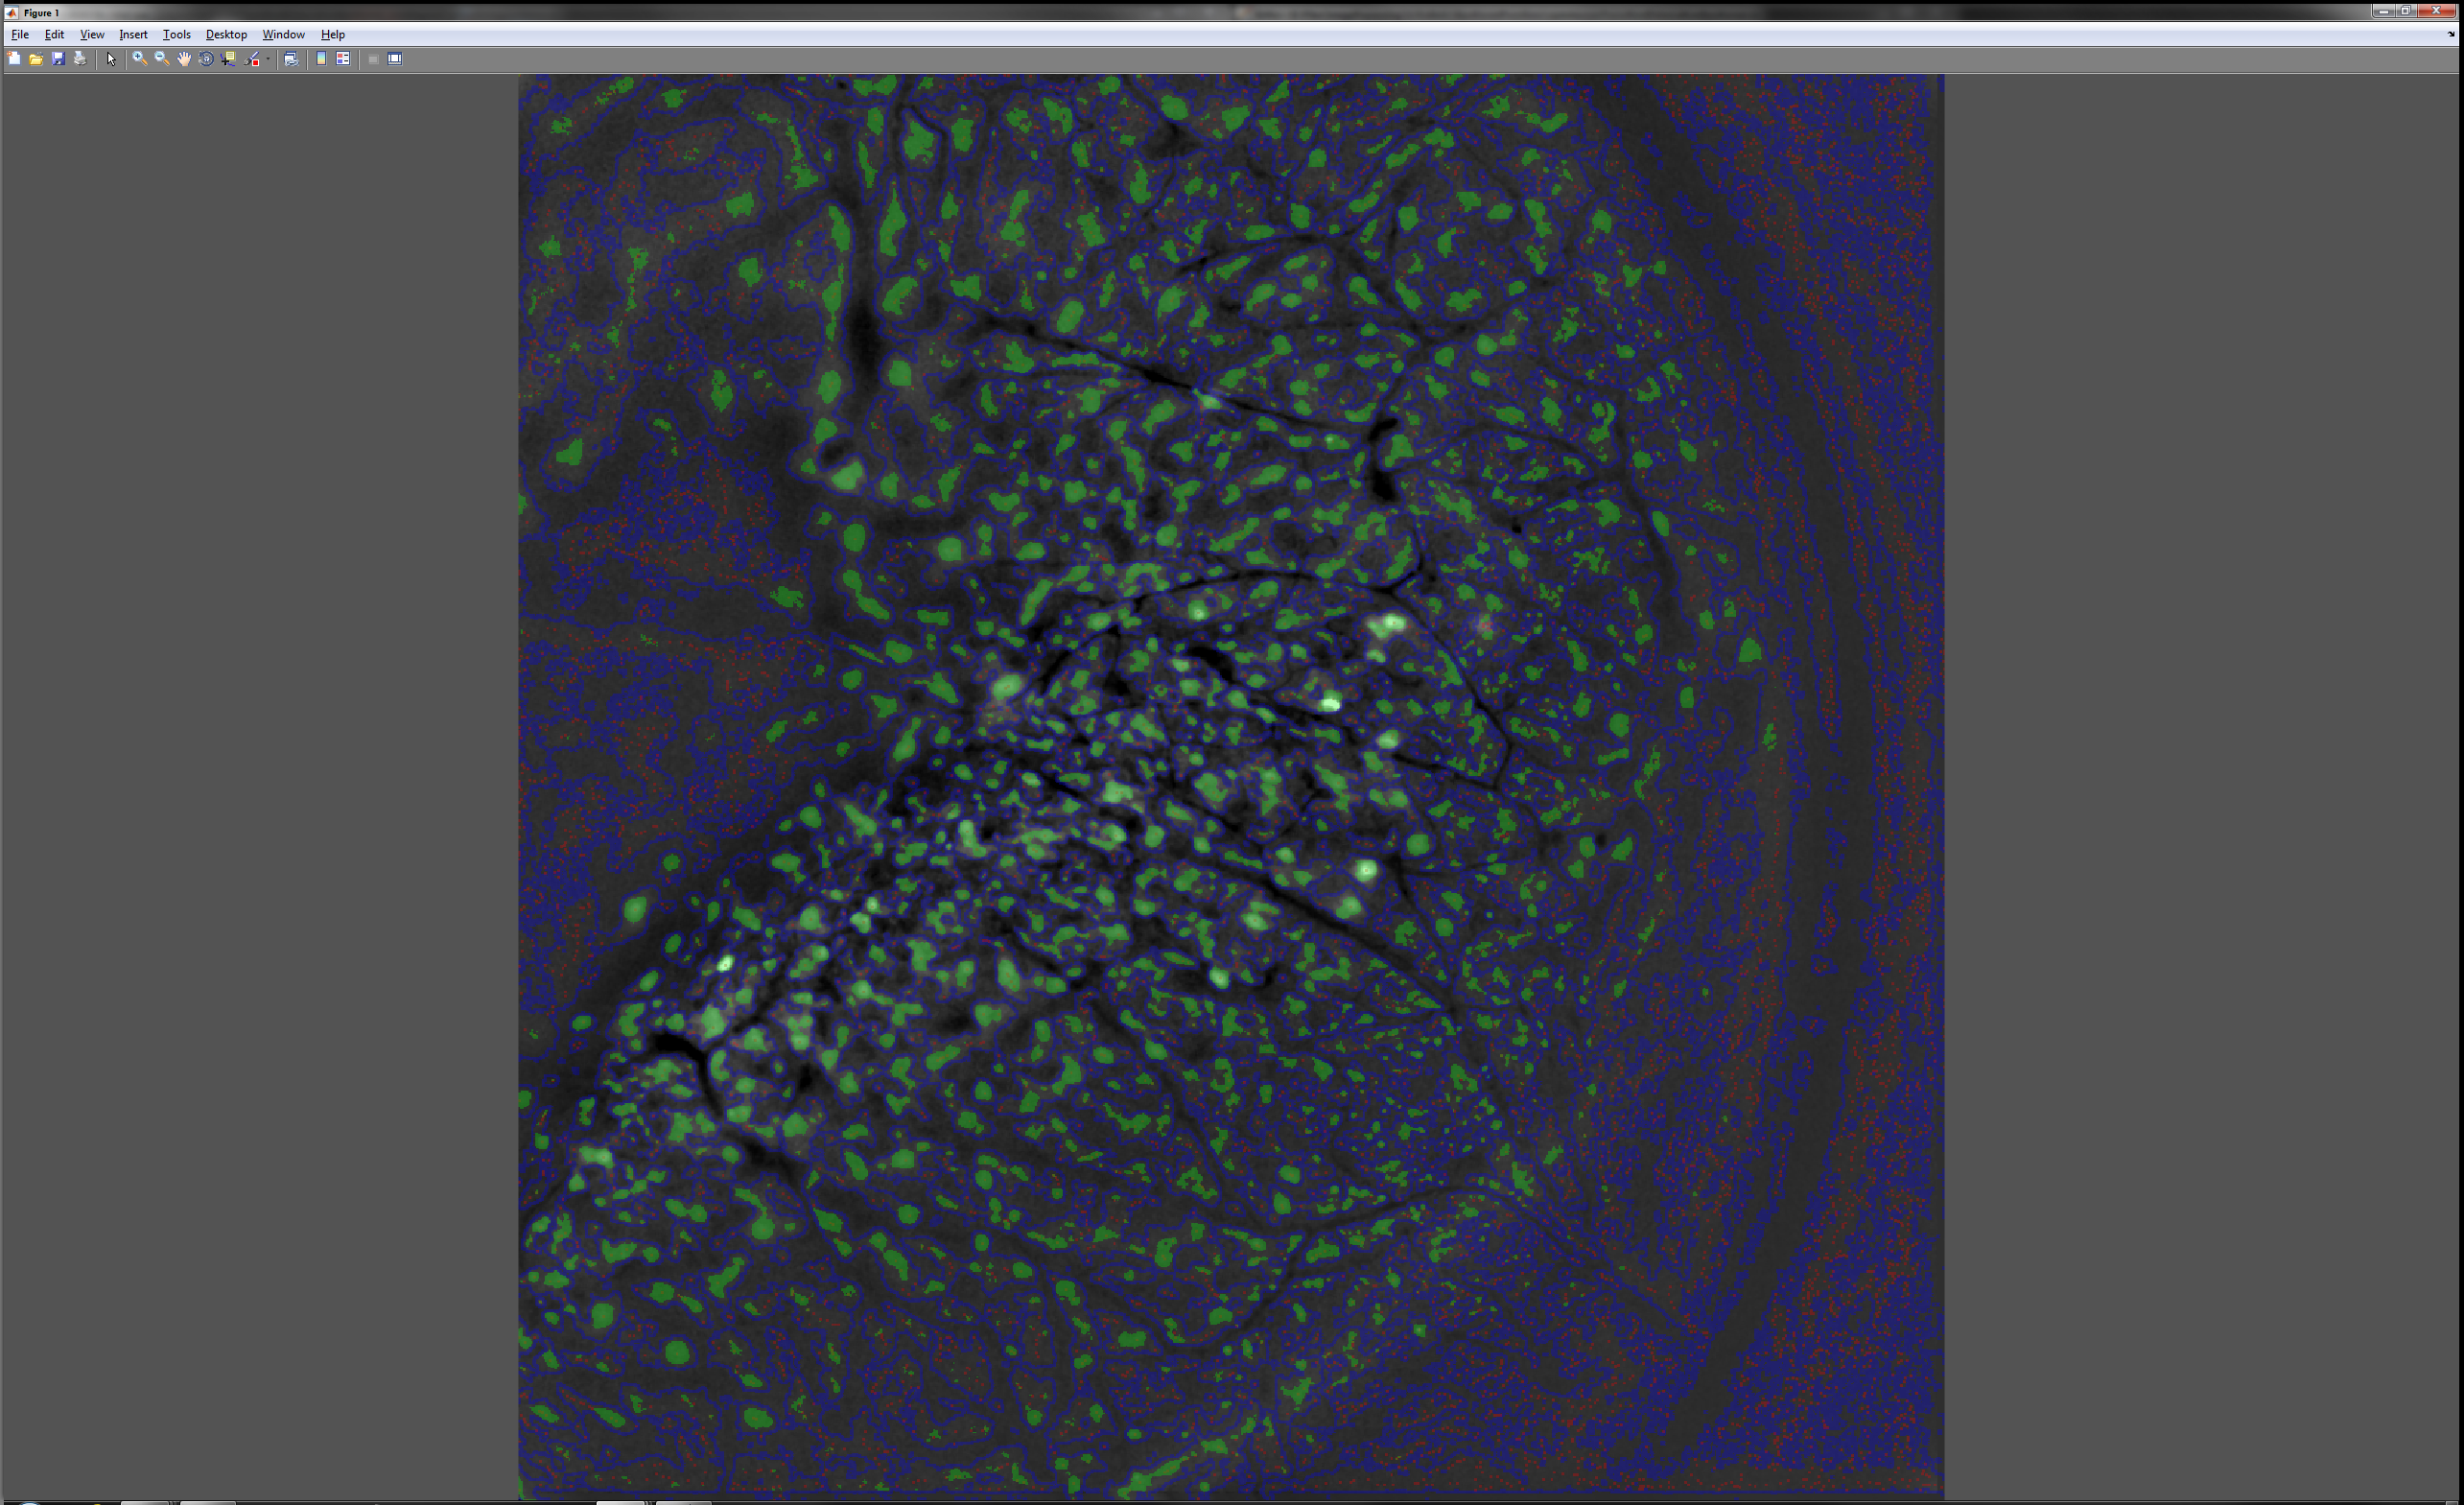
\includegraphics[height=12cm]{figures/2.png}
% 	\caption{caption}
% \end{figure}

\begin{figure}[htb]\centering
	\includegraphics[height=12cm]{figures/sw-video-processing-feature-pointwise-mutual-information.png}
	\caption{Feature generation of single motion-compensated frame using complex-valued normalized pointwise mutual information of each pixel with its local neghborhood}
\end{figure}


% \begin{figure}[htb]\centering
% 	\includegraphics[height=12cm]{figures/trgb-013.png}
% 	\caption{caption}
% \end{figure}

\begin{figure}[htb]\centering
	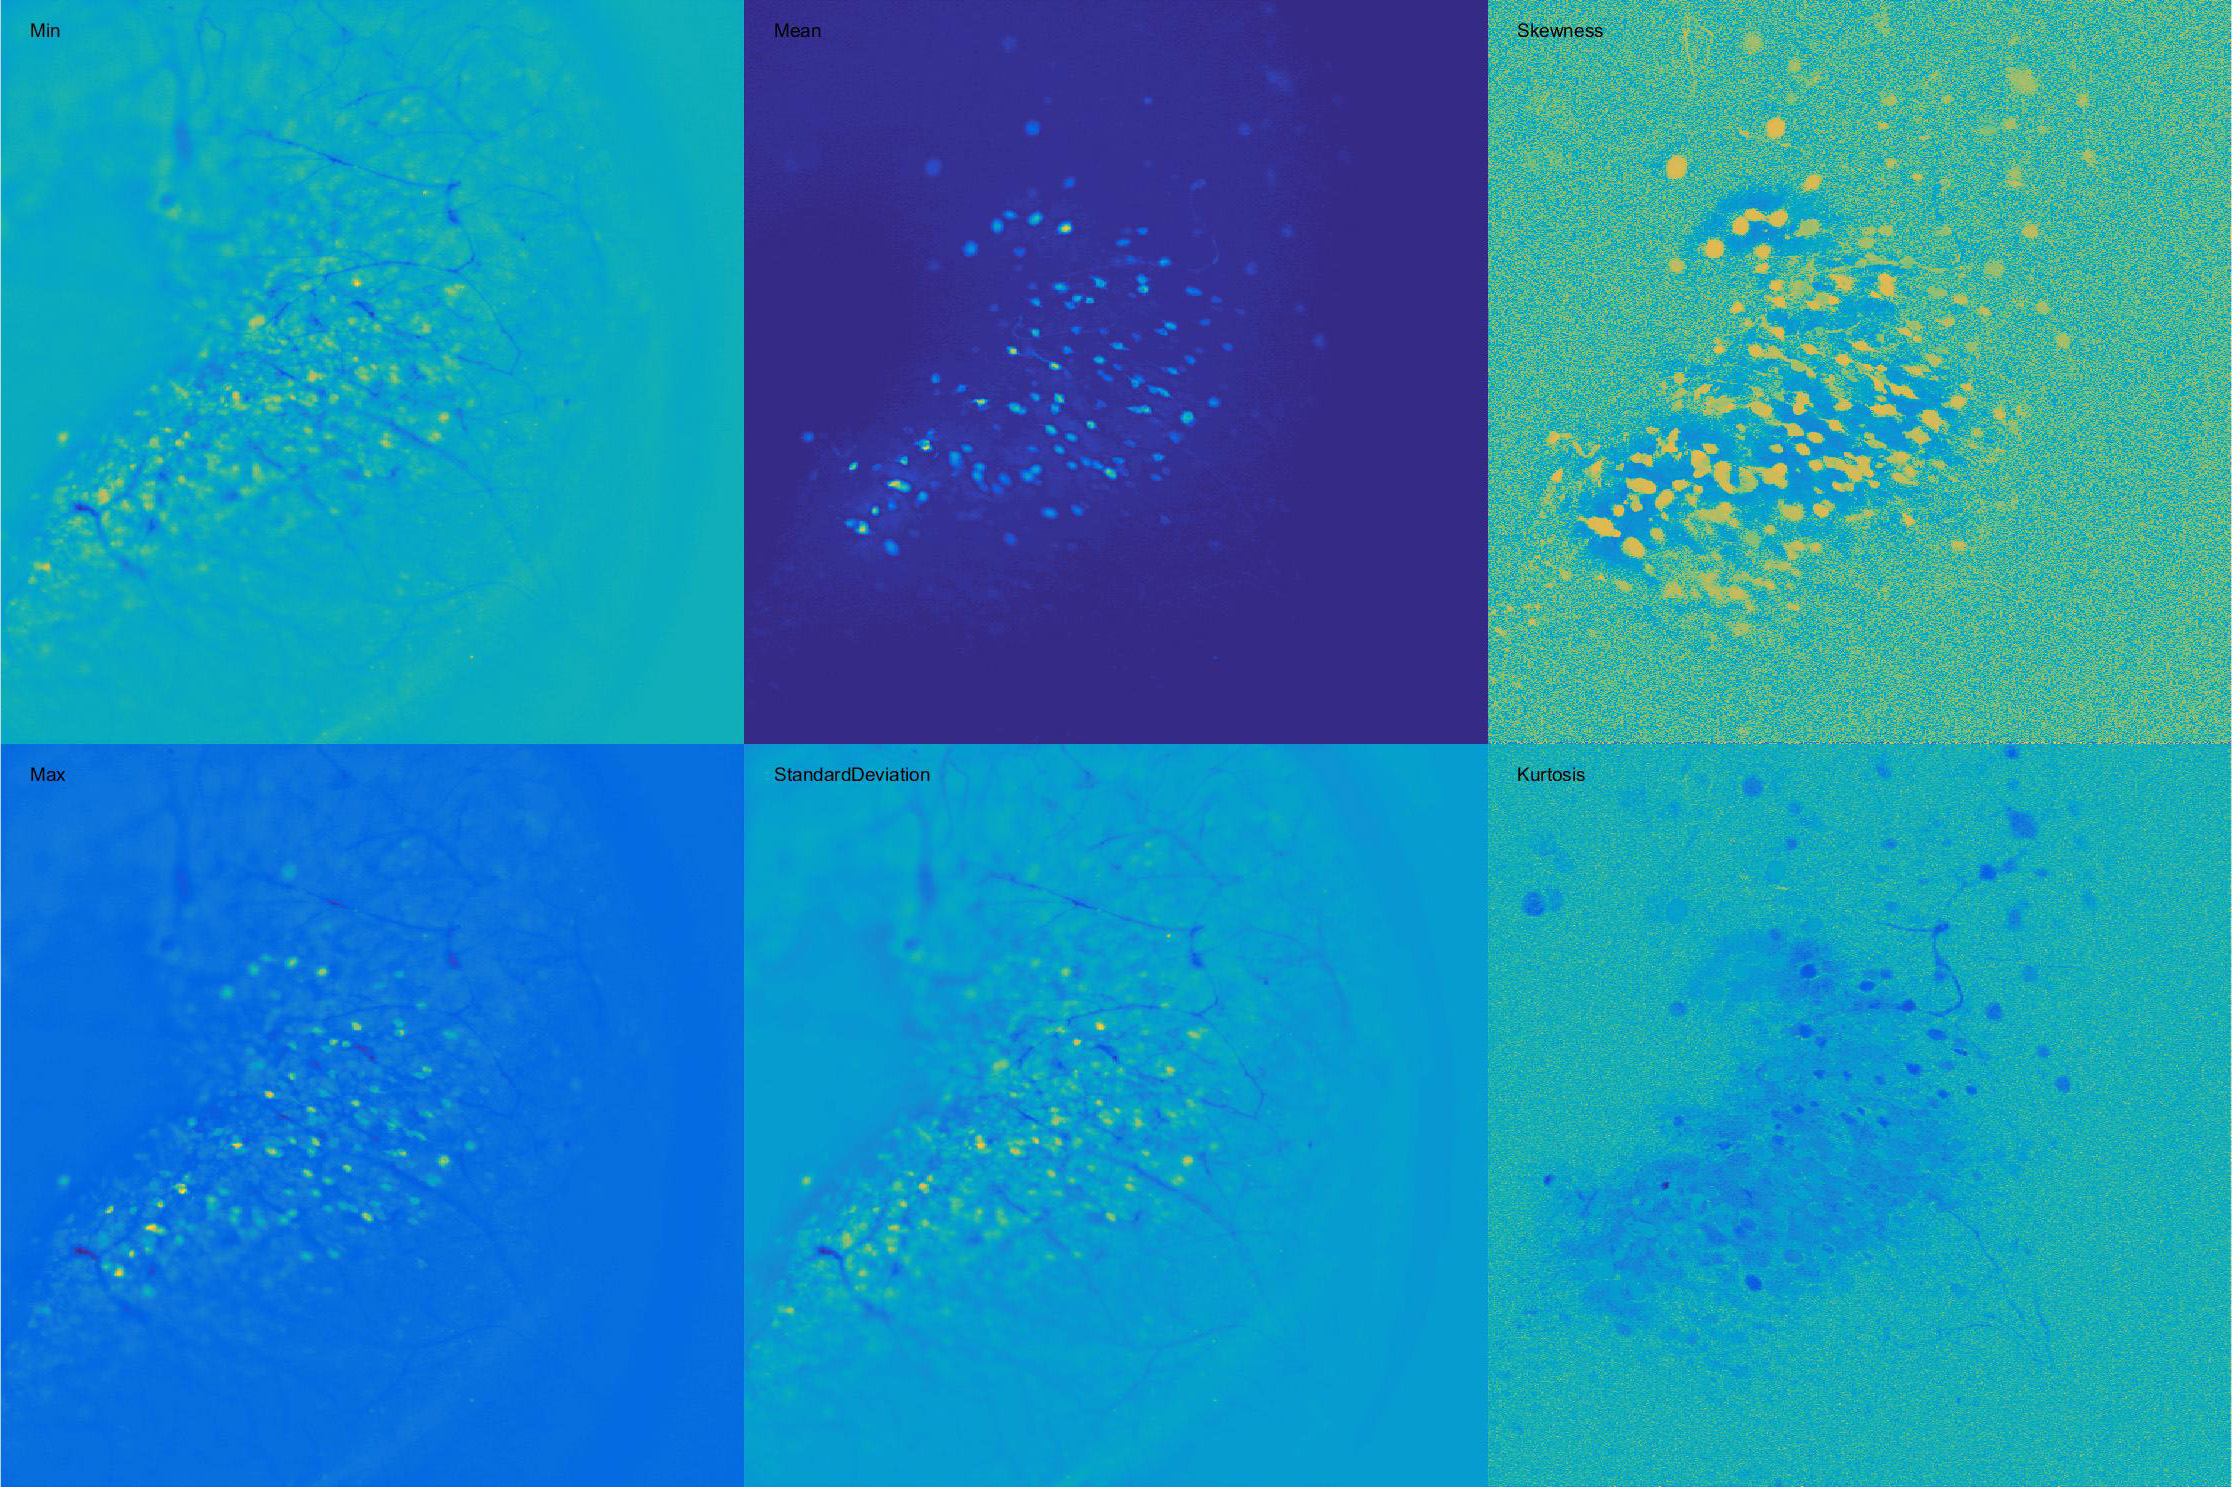
\includegraphics[width=12cm]{figures/statistics_of_128_frames_contrast_enhanced.jpg}
	\caption{Pixel-wise statistics of 128 frames (min, max, mean, standard deviation, skewness, kurtosis)}
\end{figure}


\begin{figure}[htb]\centering
	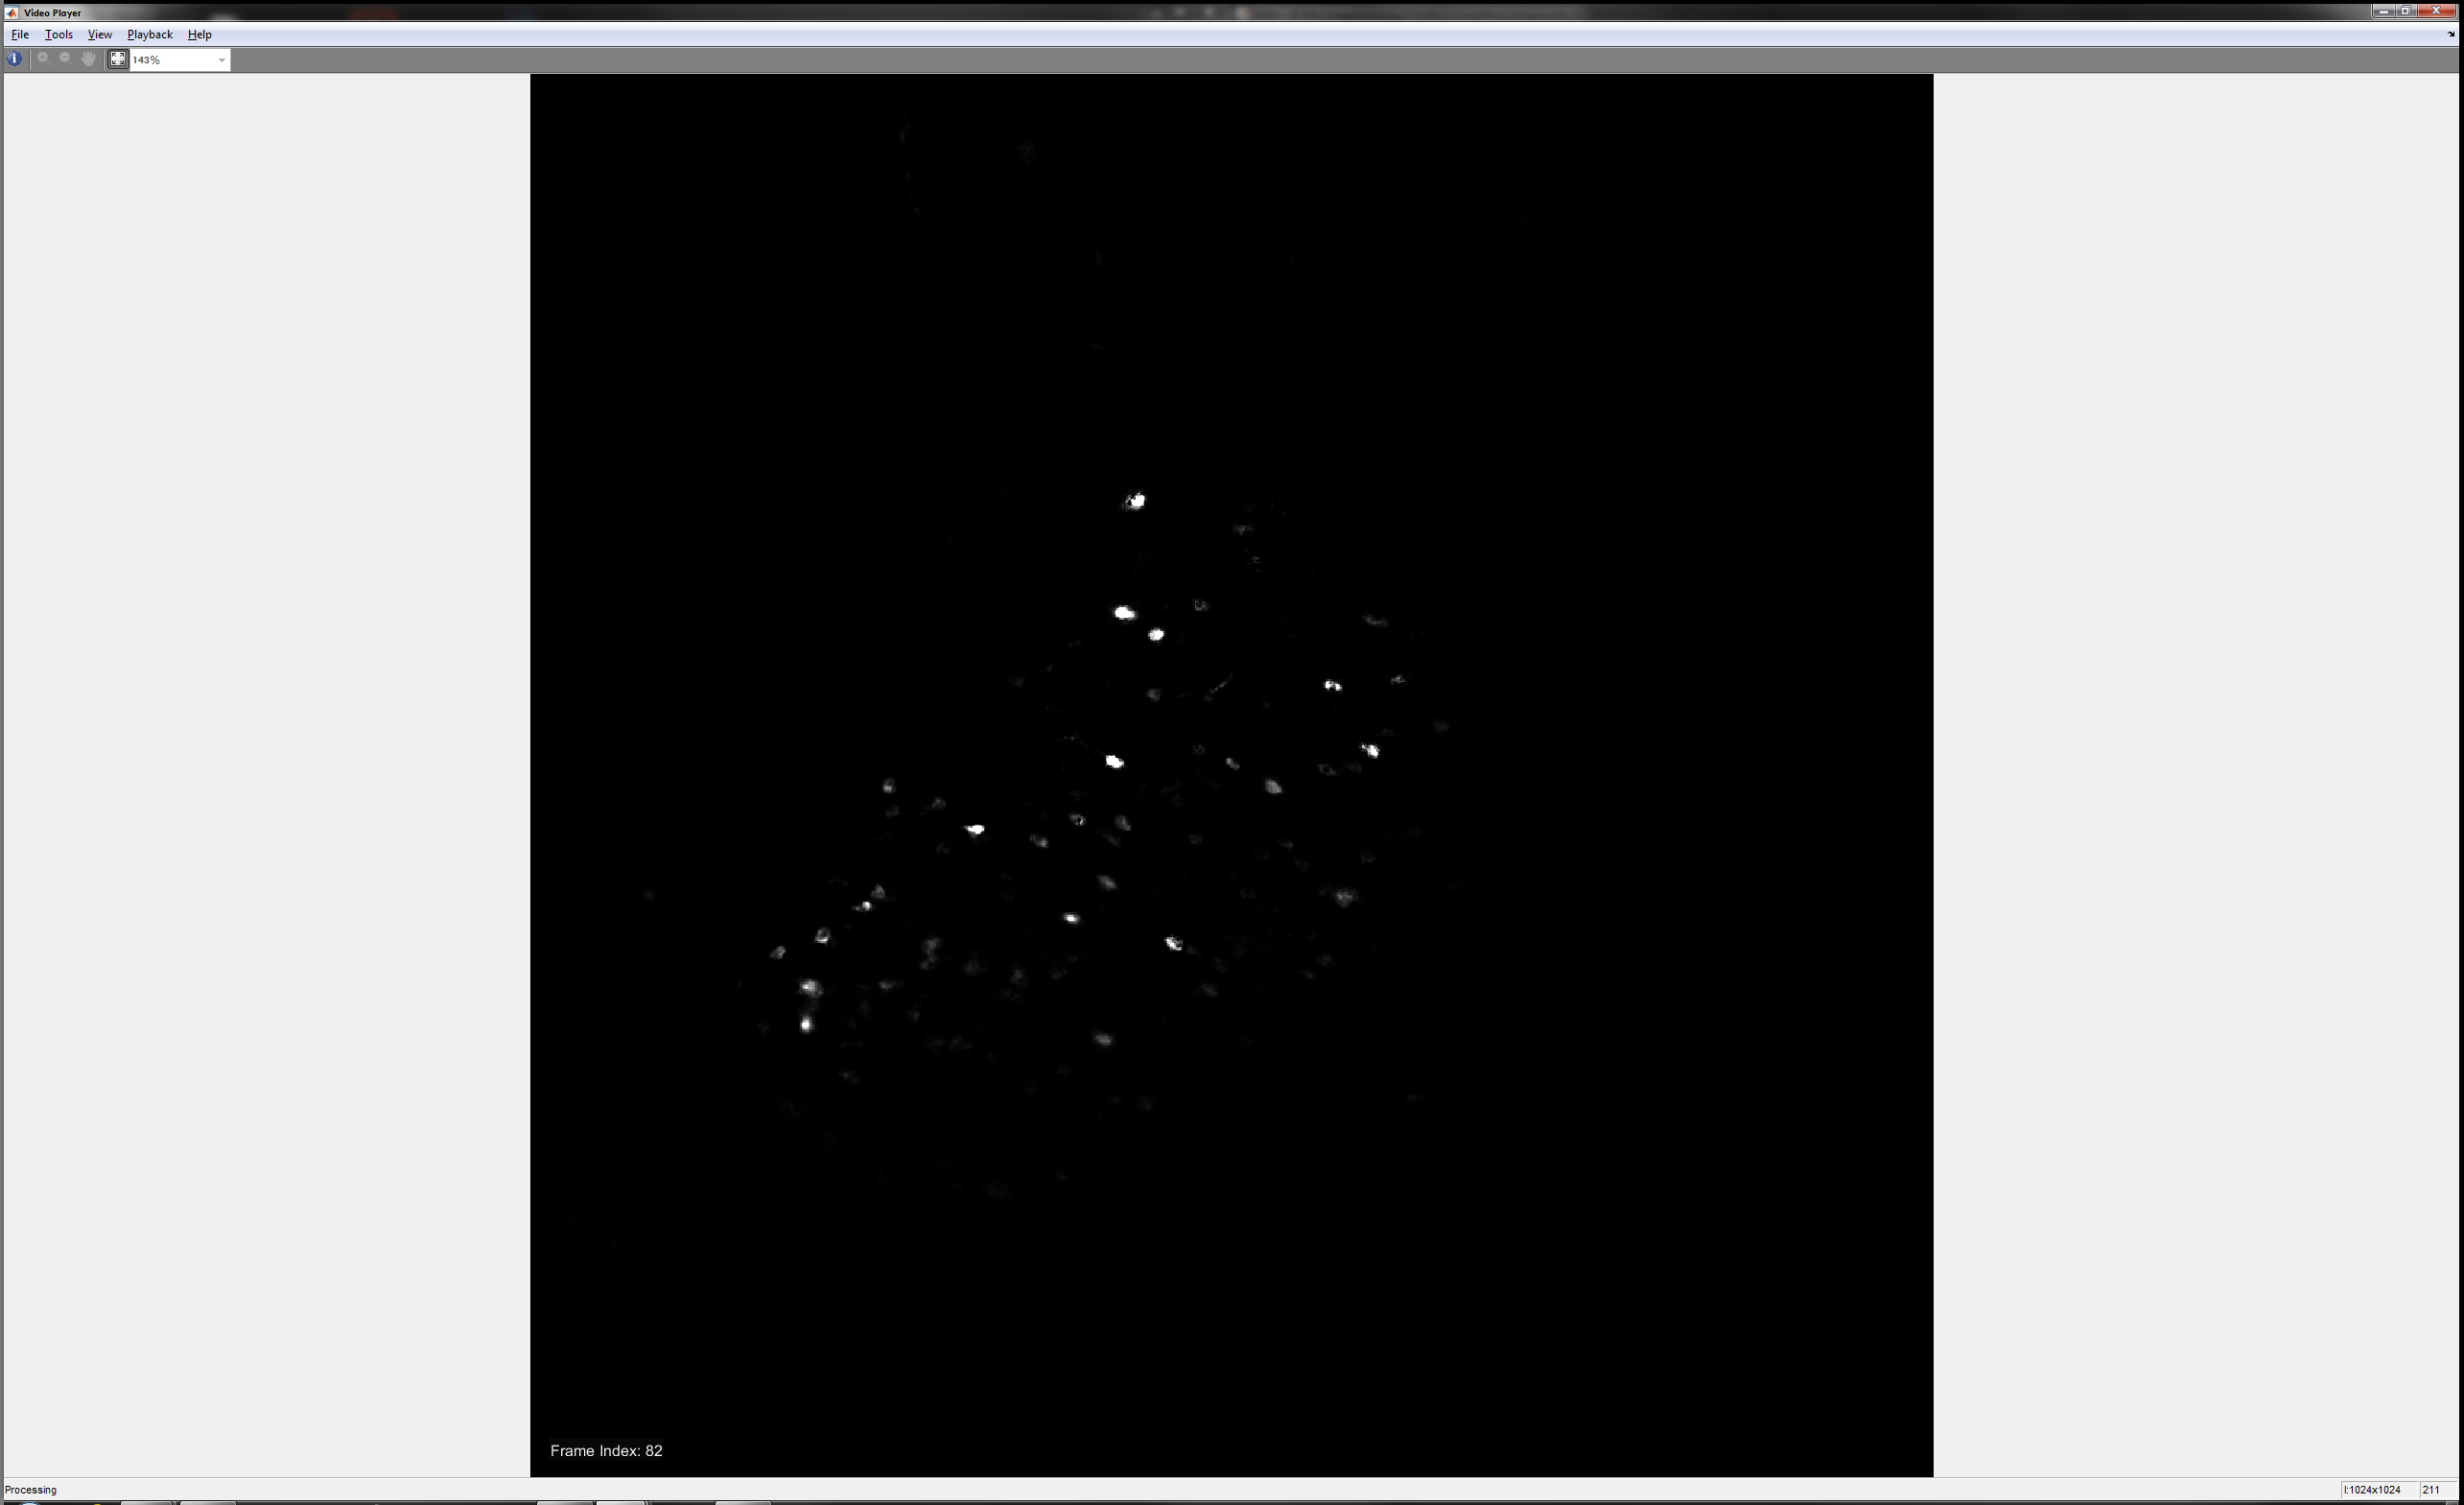
\includegraphics[width=12cm]{figures/sw-sequence-bw.png}
	\caption{Normalized differential skewness}
\end{figure}

% \clearpage


% \end{document}

\cleardoublepage{}
